\section{Exploratory Research}
\label{sec:exploratory}
We have now established some semantics of the data gathered for our research. Before diving into the data analysis, we will first quantify the data by providing the reader with some statistics.

\subsection{Overall Activity}

\begin{center}
    \begin{tabular}{|l|r|}
        \hline
        \multicolumn{2}{|c|}{Statistics} \\
        \hline
         Stories & 1,544,261 \\ 
         Submitters & 165,126 \\ 
         Upvotes & 16,668,848 \\ 
         Comments & 7,383,865 \\
         \hline
    \end{tabular}
\end{center}

An interesting remark, is that January 6th 2014 did not have any submissions. The reason for this was a long downtime of the Hacker News website
\footnote{\url{https://twitter.com/hackernewsonion/status/420068968464789505} - ``Hacker News is DOWN, but your chances of getting into YC if you know how to scale a plain text website are UP.''}.

\subsection{Upvote Distribution}
If users like a story, they can express their approval by upvoting it. These upvotes are then used to rank the stories by popularity and calculate the (currently) most popular submissions. Since the formula for determining a posts ``score'' strongly favours newly submitted stories, even stories with few upvotes can spike to the frontpage.

To enter the frontpage (the top 30), a story often needs at least ten upvotes, stories that stay on the frontpage for a longer period of time will often have over a hundred upvotes. The distribution of upvotes per story can be seen in figure~\ref{fig:distribution}. Stories placed in buckets of size 100 based on the number of upvotes they received. The graph plots the size of each bucket

Note that these graphs are scaled logarithmically: in the graph showing all posts (figure~\ref{fig:distribution_all}), 97.5\% of the stories are in the first bucket, i.e. only 2.5\% of the stories get over 100 upvotes. 

The second graph (\ref{fig:distribution_zoomed_in}) is a zoomed in version with a bucket size of 1, and shows the distribution for points with 30 upvotes or less, a set of over 1.4 million stories.

\begin{figure}[ht!]
\centering
\begin{subfigure}{.55\textwidth}
  \centering
  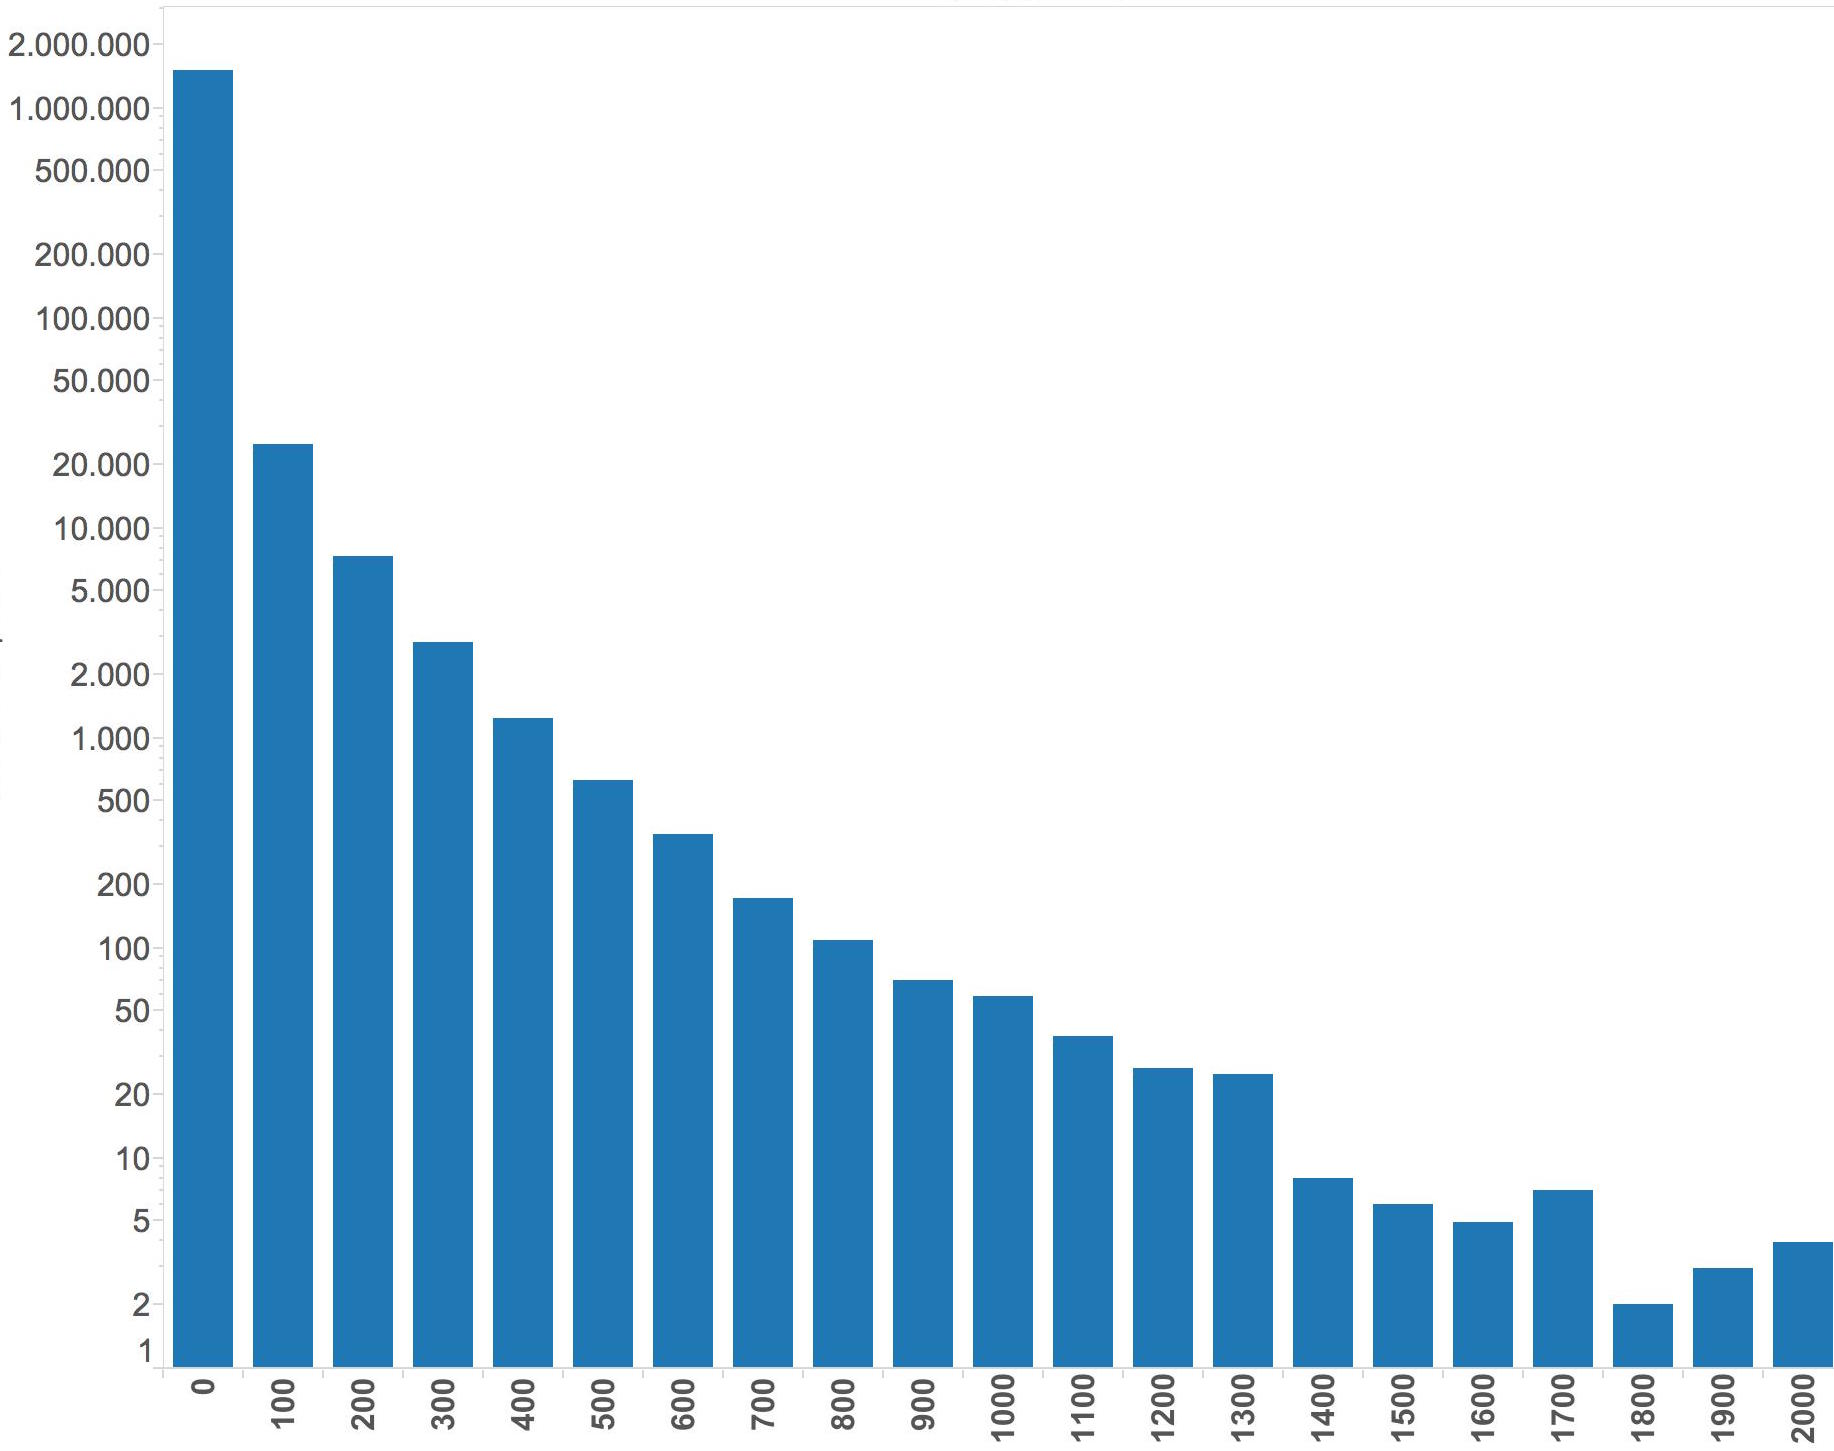
\includegraphics[height=6cm]{upvote_distribution_all}
  \caption{Distribution over all stories\\Bucket size 100}
  \label{fig:distribution_all}
\end{subfigure}%
\begin{subfigure}{.45\textwidth}
  \centering
  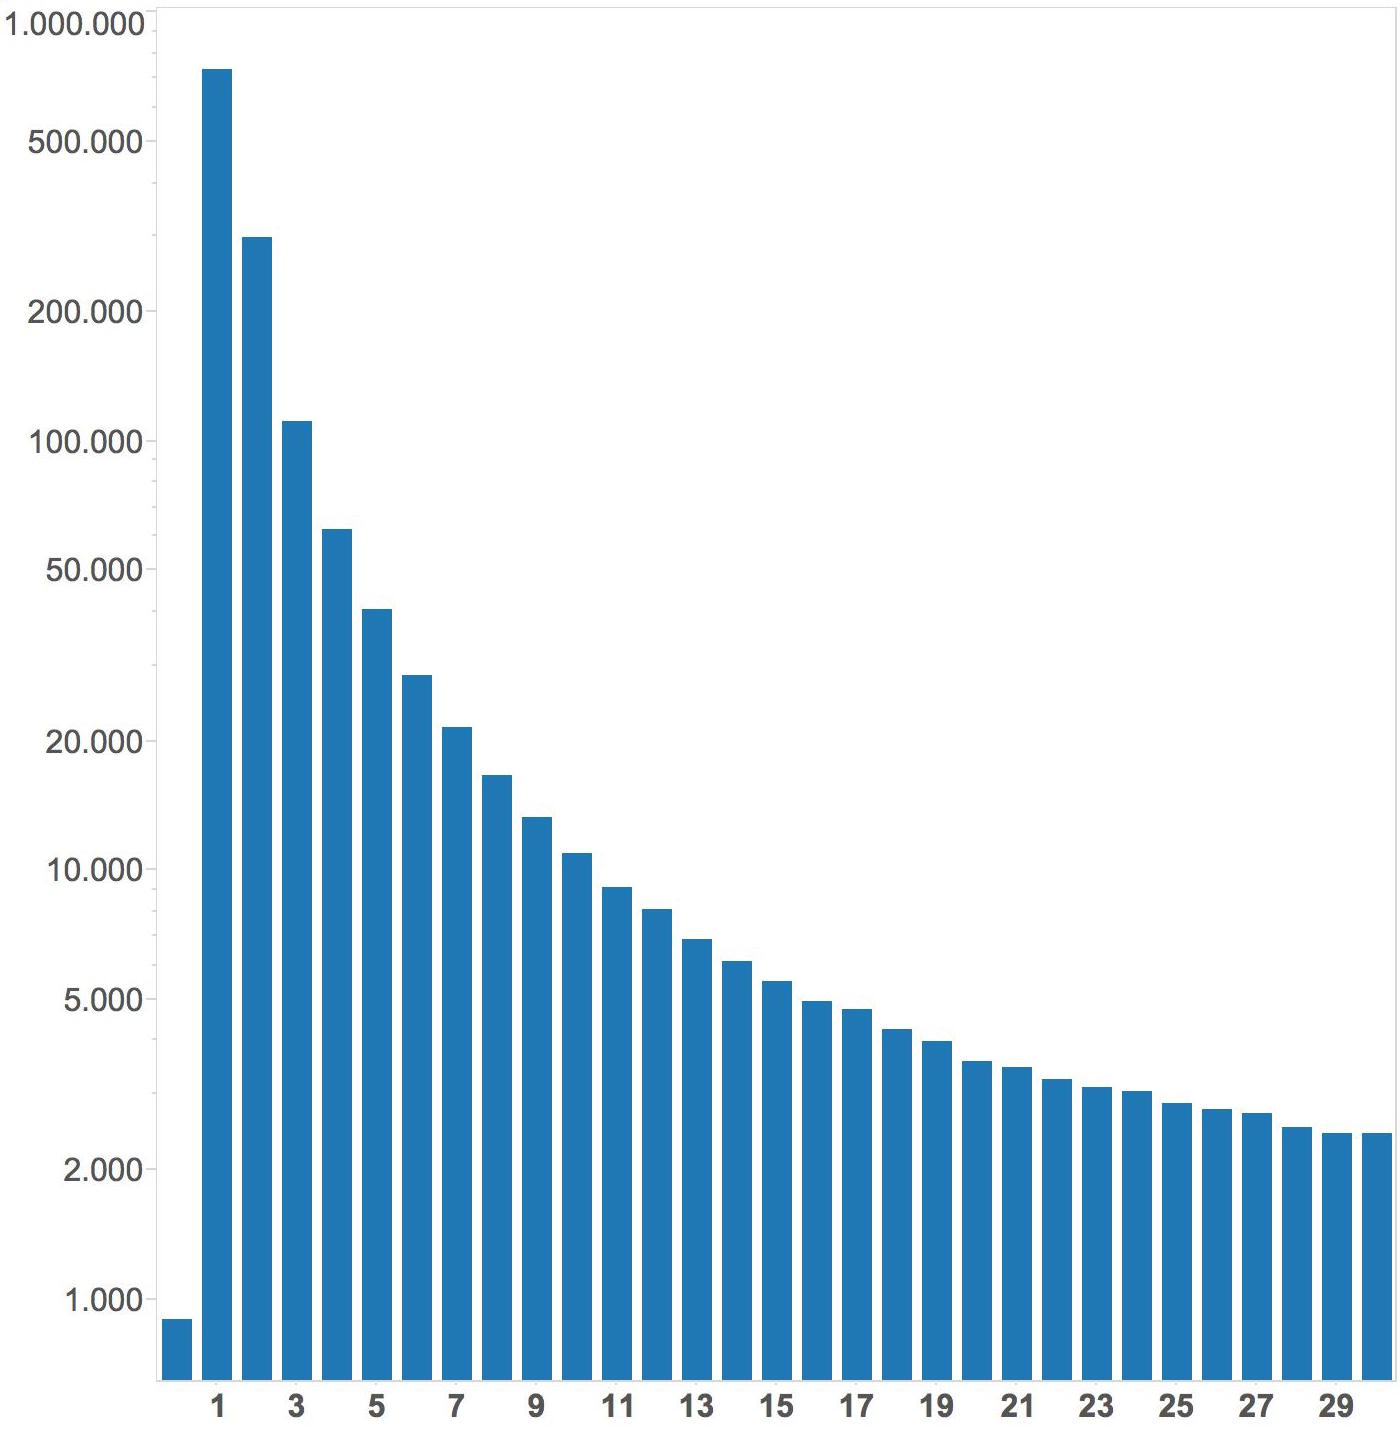
\includegraphics[height=6cm]{upvote_distribution_zoomed_in}
  \caption{Distribution over low-ranked stories\\Bucket size 1}
  \label{fig:distribution_zoomed_in}
\end{subfigure}
\caption{Distributions of upvotes over posts (log scale)}
\label{fig:distribution}
\end{figure}

There are only six stories with over 2100 upvotes. For completeness' sake, these are the stories whose popularity is quite literally ``off the charts'':
\begin{center}
    \begin{tabular}{|p{=8.5cm}|p{2cm}|}
       \hline
       \multicolumn{2}{|c|}{Most upvoted stories} \\
       \hline
       Title 																				& Points \\
       \hline
       Steve Jobs has passed away 										& 4271\\
		Tim Cook Speaks Up														& 3086\\
		2048																			& 2732\\
		Don't Fly During Ramadan											& 2617\\
		Hyperloop																		& 2549\\
		Microsoft takes NET open source and cross platform	& 2376\\
        \hline
    \end{tabular}
\end{center}

\subsection{Top Users}
In figure~\ref{fig:top10ByStories}, we show the statistics for some of the most active submitters. These statistics illustrate that Hacker News has a very active group of users. Together, this top 10 submitted 45,190 stories, which equals an average of 1.5 stories per user per day over the last 7 years.
\begin{figure}[ht!]
	\caption{Top 10 submitters by submitted stories}
	\label{fig:top10ByStories}
	\centering
	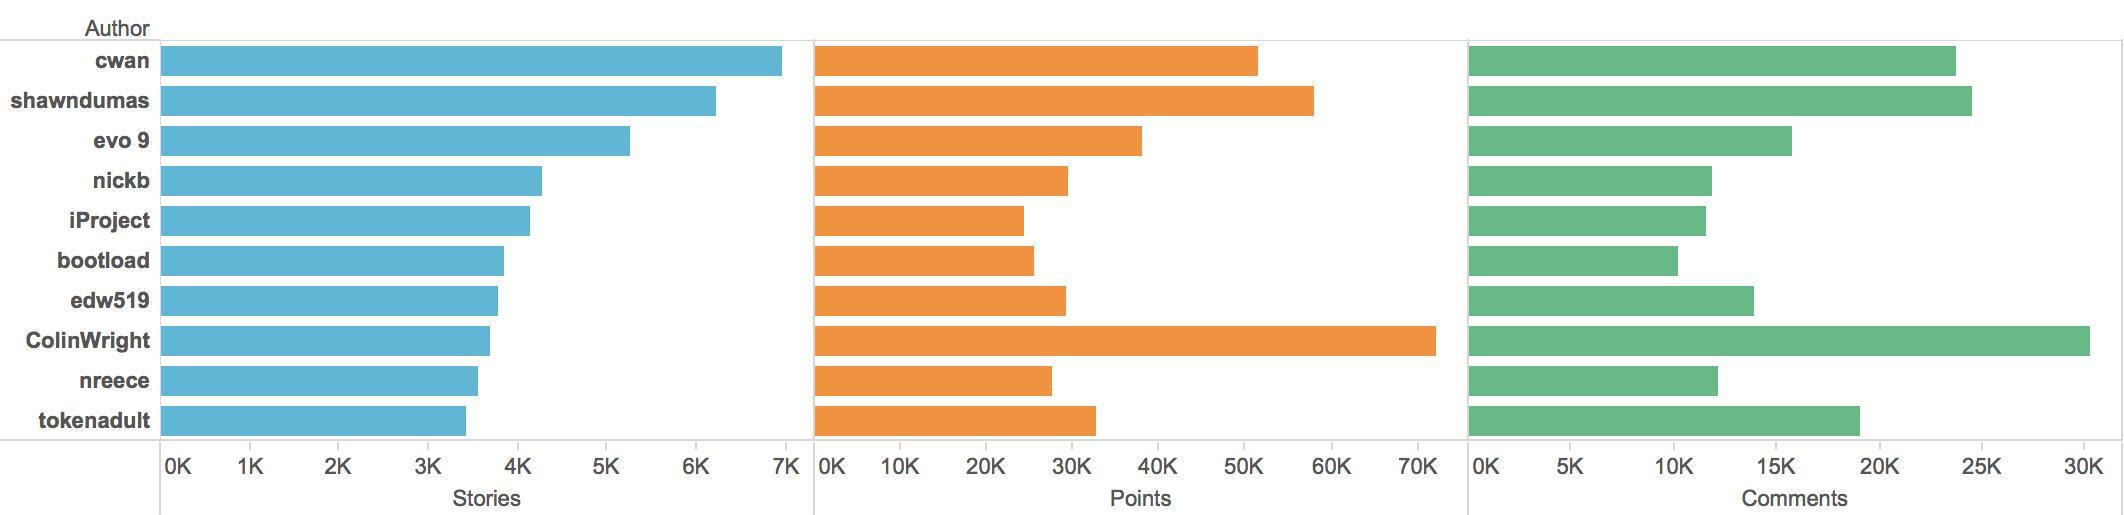
\includegraphics[width=14cm]{top10ByStories}
\end{figure}

If we take the top 10 not by the number of stories a user has submitted but by the number of comments his or her stories have received, we get the rankings in figure~\ref{fig:top10ByComments}.

\begin{figure}[ht!]
	\caption{Top 10 submitters by received comments}
	\label{fig:top10ByComments}
	\centering
	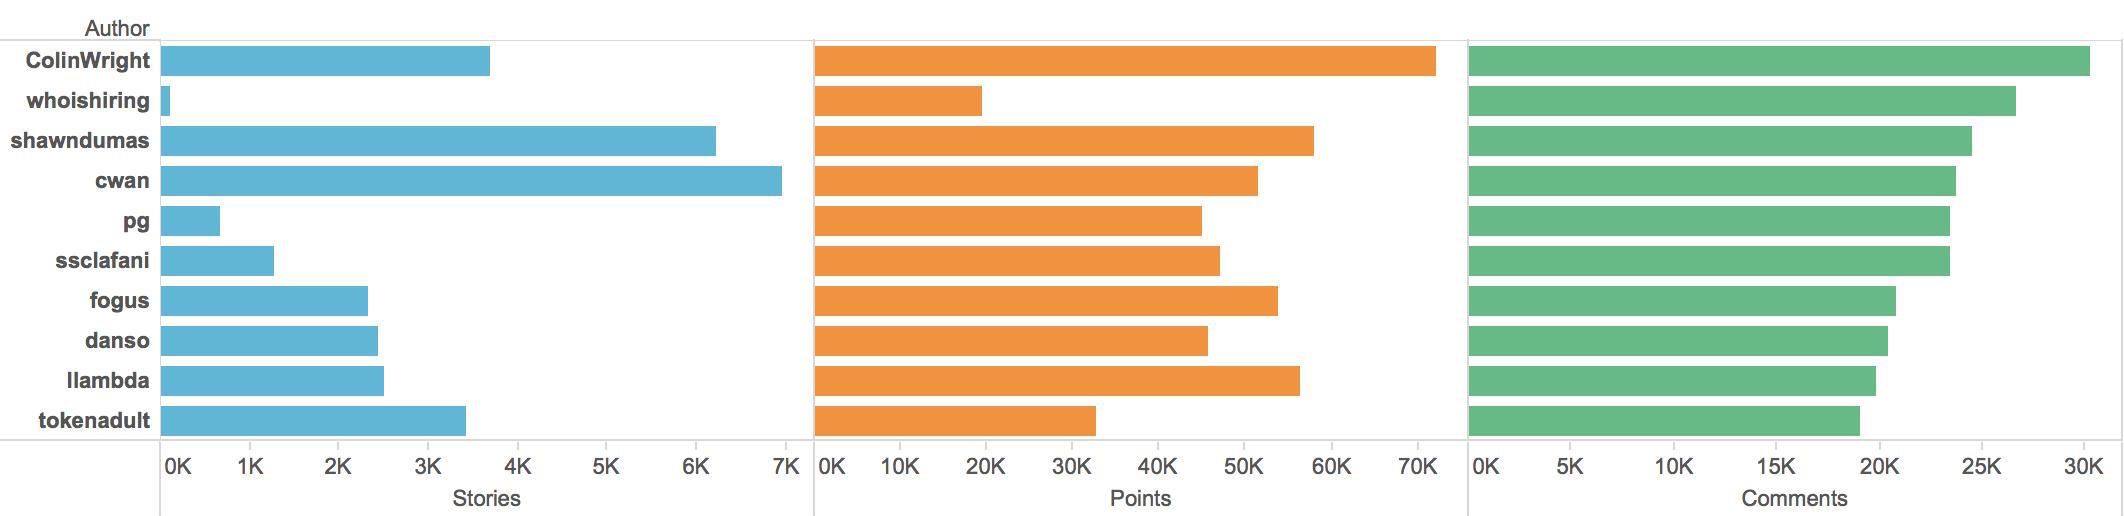
\includegraphics[width=14cm]{top10ByComments}
\end{figure}

The interesting second place in this top 10 is user ``\_whoishiring``. This user has almost no posts (a mere 114) but received 26,649 comments. Experienced Hacker News readers may have already expected this, for this user starts a monthly thread where companies can post job offers and others can respond to these. As such, the user only posts one story per month but its stories are discussed very actively.

\subsection{Top Domains}
As already stated in the description of the dataset, many of the stories are links to external sites. To provide some insights into which sites attract a lot of attention from the Hacker News community, we made three top ten lists that rank the sites by the same criteria as we did in the previous section: by number of stories, by points and by number of comments.

\begin{center}
    \begin{tabular}{|p{4.5cm}|p{=5cm}|p{5cm}|}
       \hline
       \multicolumn{3}{|c|}{Most popular domains} \\
       \hline
       By Number of Stories 			& By Points 									& By Comments \\
       \hline
       techcrunch.com (27.711) 	& github.com (400.373)		       & techcrunch.com (172.854) \\
		github.com (26.596) 			& techcrunch.com (365.207) 	   & nytimes.com (153.471) \\
		youtube.com (21.977) 		& nytimes.com (287.234)		   & github.com (127.812) \\
		nytimes.com (18.125) 		& arstechnica.com (176.633)	   & arstechnica.com (80.666) \\
		medium.com (14.172) 		& wired.com (161.698)		  	   & wired.com (75.406) \\
		arstechnica.com (12.657) 	& medium.com (132.468)		   & washingtonpost.com (56.257) \\
		wired.com (10.867) 			& bbc.co.uk (98.031)		  		   & medium.com (53.924) \\
		bbc.co.uk (8.118) 				& washingtonpost.com (97.537) & bbc.co.uk (51.828) \\
		en.wikipedia.org (7.058) 		& youtube.com (96.339)		  	   & theatlantic.com (41.530) \\
		businessinsider.com (6.877) & theatlantic.com (77.628)	   & online.wsj.com (36.729) \\
        \hline
    \end{tabular}
\end{center}

These rankings provide some insights into what types on news are popular. The big geeky news sites (Techcrunch, Ars Technica and Wired) are present and are about as popular as the big newspapers (NY Times, BBC, Washington Post). 

The high ranking of github.com (a code hosting site, \textit{not} a news site) can be explained by the large number of open source projects hosted on GitHub that submit links to new versions and press releases on Hacker News. Some examples of these projects are Facebook's React framework, Twitter's Bootstrap, SQLite and io.js. 

Notably, GitHub's competitors (e.g. BitBucket, GitLab and Beanstalk) do not show up in these rankings. This demonstrates GitHub's overpowering popularity in the code hosting market, at least in the open source community.

% TODO where do we put this part...
In the top lists given above, we have provided the number of articles, points and comments on groups of articles. The strong similarity between the different methods of ranking indicates a strong correlation between how well a story scores on various features. This is in line with what one might expect: people post, like and comment most of things they consider most interesting.

\subsection{Measuring popularity}
First and foremost, our popularity must account for different lengths of months and a smaller userbase in the early years of Hacker News. To do so, we must use relative scores per month, rather than providing absolute number.

We have decided to base our popularity measure on all three features we used for the rankings above: number of articles, number of upvotes and number of comments. If a topic receives 2\% of the arcticles, 2\% of the upvotes and 5\% of the comments, the popularity score is 3\% (the average of the three).

To give a formal definition: let $S_m$ be the set of all stories in month $m$ and $T_i$ all stories in the topic number $i$. With these two definitions, $S_m \cup T_i$ is the set of all stories on a topic $i$ in month $m$. Furthermore, let $s_u$ (resp. $s_c$) be the number of upvotes (resp. comments) story $s$ has received. Then, given a topic id $i$ and a month $m$, the score for that topic in that month is:

$$
	score(i, m) = 
		\frac{1}{3} \frac{|S_m \cup T_i|}{|S_m|} + 
		\frac{1}{3} \frac{\sum_{s \in S_m \cup \in T_i} s_u}{\sum_{s \in S_m} s_u}  + 
		\frac{1}{3} \frac{\sum_{s \in S_m \cup \in T_i} s_c}{\sum_{s \in S_m} s_c}
$$
